\documentclass[11pt,a4paper]{article}

\usepackage[a4paper,margin=2.5cm]{geometry}
\usepackage[utf8]{inputenc}
\usepackage[T1]{fontenc}
\usepackage{lmodern}
\usepackage{microtype}
\usepackage{xcolor}
\usepackage{graphicx}
\usepackage{booktabs}
\usepackage{longtable}
\usepackage{array}
\usepackage{enumitem}
\usepackage{listings}
\usepackage{tikz}
\usetikzlibrary{arrows.meta,positioning,fit,backgrounds}
\usepackage{hyperref}
\usepackage{amsmath}
\usepackage{titlesec}
\usepackage{parskip}
\usepackage{fancyhdr}

\definecolor{codebg}{RGB}{245,245,245}
\definecolor{codekw}{RGB}{0,90,150}
\definecolor{codecomment}{RGB}{110,110,110}
\definecolor{coderule}{RGB}{200,200,200}

\lstdefinestyle{base}{
    backgroundcolor=\color{codebg},
    basicstyle=\ttfamily\footnotesize,
    commentstyle=\color{codecomment}\itshape,
    keywordstyle=\color{codekw}\bfseries,
    frame=single,
    rulecolor=\color{coderule},
    breaklines=true,
    breakatwhitespace=false,
    showstringspaces=false,
    tabsize=2,
    xleftmargin=1em,
    xrightmargin=1em,
    framesep=6pt
}
\lstset{style=base}
\lstdefinelanguage{yaml}{
    keywords={},
    sensitive=false,
    comment=[l]{\#},
    morestring=[b]',
    morestring=[b]"
}

\hypersetup{
    colorlinks=true,
    linkcolor=blue!50!black,
    urlcolor=blue!50!black,
    citecolor=blue!50!black,
    pdftitle={Air Hockey Robot -- Technical Documentation},
    pdfauthor={Air Hockey Robot Project}
}

\titleformat{\section}{\normalfont\Large\bfseries}{\thesection}{1em}{}
\titleformat{\subsection}{\normalfont\large\bfseries}{\thesubsection}{1em}{}

\pagestyle{fancy}
\fancyhf{}
\fancyhead[L]{Air Hockey Robot}
\fancyhead[R]{\leftmark}
\fancyfoot[C]{\thepage}
\renewcommand{\headrulewidth}{0.4pt}

\newcommand{\code}[1]{\texttt{\detokenize{#1}}}
\newcommand{\topicname}[1]{\texttt{\detokenize{#1}}}
\newcommand{\pkg}[1]{\textbf{\texttt{\detokenize{#1}}}}

\title{\textbf{Autonomous Air Hockey Robot} \\ \large ROS~2 Workspace -- Technical Documentation}
\author{}
\date{}

\begin{document}

\maketitle
\thispagestyle{empty}

\begin{abstract}
\noindent
This document describes the software architecture of a ROS~2 based autonomous
air hockey robot built around an ABB IRB1200 industrial arm. An overhead
camera streams video of the table to a perception pipeline that locates the
puck using AprilTag/ArUco fiducial markers, a Kalman-filter based predictor
that estimates where the puck will enter the robot's defense zone (including
wall bounces), and a motion controller that drives the arm's tool-center
point over ABB's Externally Guided Motion (EGM) protocol to block or strike
the puck. A companion Gazebo simulation package reproduces the physical
table, puck, camera and robot so that the exact same perception and control
code can be developed and tested without the physical hardware.
\end{abstract}

\tableofcontents

% ============================================================
\section{System Overview}
% ============================================================

The project is a ROS~2 (Humble) colcon workspace with four packages under
\code{src/}:

\begin{itemize}
  \item \pkg{air_hockey_robot_msgs} -- Custom ROS~2 message definitions
        shared by every other package in the pipeline.
  \item \pkg{pc_node} -- The C++ ``brain'' of the robot: perception,
        trajectory prediction and robot motion control. Runs on a PC (not
        the Raspberry Pi that hosts the camera).
  \item \pkg{air_hockey_sim} -- A Gazebo (\code{ros_gz}) simulation of the
        physical table, puck and IRB1200 robot, used as a drop-in
        replacement for the real camera/robot during development.
  \item \pkg{abb_ros2} -- An external dependency (ABB's ROS~2 support
        packages, e.g.\ \code{abb_irb1200_support}) that must be cloned
        into \code{src/} separately; it supplies the robot's URDF/mesh
        description used by \pkg{air_hockey_sim}. It is not vendored in
        this repository.
\end{itemize}

Outside the ROS~2 workspace, the repository also contains:

\begin{itemize}
  \item \code{robot/} -- RAPID modules (\code{main.mod}, \code{EGM.mod})
        that run directly on the ABB controller and set up the EGM
        streaming session.
  \item \code{calibration.yml}, \code{table_markers.yml} -- camera
        intrinsics and measured physical marker positions used by
        \code{perception_node}.
  \item \code{markers_png/} -- printable AprilTag~16h5 marker images
        (the puck marker and the eight table-band markers).
  \item \code{table_models/} -- 3D geometry (\code{.obj}) of the
        countertop, cushion band and puck.
  \item \code{build_script.sh}, \code{run_pc_nodes.sh} -- convenience
        scripts to build the workspace and launch the three PC nodes with
        logging.
\end{itemize}

A camera (either the real overhead camera, streamed in from a Raspberry
Pi, or the simulated Gazebo camera) is the only sensor input; there is no
separate puck-color or shape detector -- the puck itself carries an
AprilTag~16h5 marker, and eight more markers fixed around the table band
give the homography that converts pixel coordinates into physical
table-frame millimetres.

% ============================================================
\section{Data Flow and Node Pipeline}
% ============================================================

\begin{figure}[h]
\centering
\resizebox{\linewidth}{!}{%
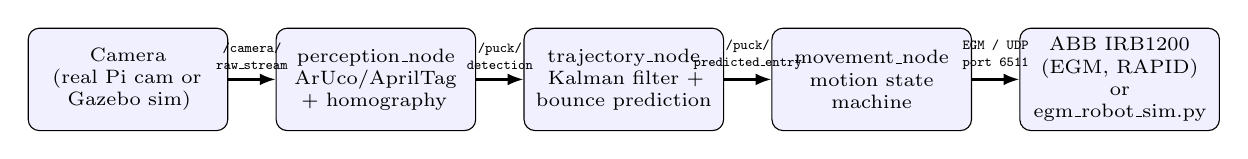
\begin{tikzpicture}[
  node distance=0.5cm and 0.6cm,
  box/.style={draw, rounded corners, fill=blue!6, align=center, minimum height=1.3cm, text width=2.3cm, font=\scriptsize},
  topic/.style={font=\tiny\ttfamily, align=center},
  arr/.style={-{Latex[length=2mm]}, thick}
]
  \node[box] (cam) {Camera\\(real Pi cam or\\Gazebo sim)};
  \node[box, right=of cam] (perc) {perception\_node\\ArUco/AprilTag\\+ homography};
  \node[box, right=of perc] (traj) {trajectory\_node\\Kalman filter +\\bounce prediction};
  \node[box, right=of traj] (mov) {movement\_node\\motion state\\machine};
  \node[box, right=of mov] (robot) {ABB IRB1200\\(EGM, RAPID)\\or egm\_robot\_sim.py};

  \draw[arr] (cam) -- node[topic, above]{/camera/\\raw\_stream} (perc);
  \draw[arr] (perc) -- node[topic, above]{/puck/\\detection} (traj);
  \draw[arr] (traj) -- node[topic, above]{/puck/\\predicted\_entry} (mov);
  \draw[arr] (mov) -- node[topic, above]{EGM / UDP\\port 6511} (robot);
\end{tikzpicture}%
}
\caption{End-to-end pipeline: image capture $\rightarrow$ marker-based
perception $\rightarrow$ trajectory prediction $\rightarrow$ motion
control $\rightarrow$ robot.}
\end{figure}

The list below summarises every topic exchanged between the three
\pkg{pc_node} executables (message type and publisher in parentheses).

\begin{description}[style=nextline,leftmargin=1.6cm,font=\ttfamily\bfseries]
\item[\topicname{/camera/raw_stream}] (\code{PuckState}, published by the
      camera driver / \code{camera_sim_bridge.py}) -- Timestamped
      compressed JPEG frame from the overhead camera.
\item[\topicname{/puck/detection}] (\code{PuckDetection}, published by
      \code{perception_node}) -- Puck's table-frame position (mm) plus raw
      pixel coordinates, or \code{is_detected=false}.
\item[\topicname{/puck/predicted_entry}] (\code{PredictedEntry}, published
      by \code{trajectory_node}) -- Predicted puck position/velocity,
      predicted entry point and time into the defense zone, confidence,
      and a visualization path (post-bounce waypoints).
\item[\topicname{/puck/defense_zone}] (\code{Float32MultiArray}, published
      by \code{trajectory_node}) -- Bounding box of the active defense
      zone, for visualization/telemetry.
\item[\topicname{/robot/sent_position}] (\code{Float32MultiArray},
      published by \code{movement_node}) -- Last commanded table-frame
      $(x,y)$ target sent to the robot.
\item[\topicname{/robot/actual_position}] (\code{Float32MultiArray},
      published by \code{movement_node}) -- Robot's actual table-frame
      position, from EGM feedback.
\item[\topicname{/robot/detection_to_send_latency_ms}] (\code{Float32},
      published by \code{movement_node}) -- End-to-end latency from puck
      detection to EGM command send.
\item[\topicname{/robot/target_accepted}] (\code{Bool}, published by
      \code{movement_node}) -- Whether the latest predicted entry was
      actually acted on (not rejected by the gating logic).
\end{description}

% ============================================================
\section{Repository Layout}
% ============================================================

\begin{lstlisting}[language=bash]
air_hockey_robot_ros/
  src/
    air_hockey_robot_msgs/   # custom .msg definitions
      msg/
        PuckState.msg
        PuckDetection.msg
        PredictedEntry.msg
    pc_node/                 # perception + prediction + motion control (C++)
      app/                   # executable entry points (main.cpp per node)
      src/, include/         # node/library implementations
      egm/                   # ABB EGM protobuf definition (egm.proto)
    air_hockey_sim/          # Gazebo simulation (ros_gz)
      launch/                # air_hockey_table.launch.py
      models/                # table, puck, paddle SDF models
      worlds/                # air_hockey_table.sdf
      scripts/               # egm_robot_sim.py, camera_sim_bridge.py, ...
      config/                # sim calibration + Gazebo<->ROS joint bridge config
    abb_ros2/                # EXTERNAL: clone ABB's ROS 2 packages here
                              # (e.g. abb_irb1200_support) - not vendored
  robot/                     # RAPID modules run on the ABB controller
    main.mod
    EGM.mod
  calibration.yml            # OpenCV camera intrinsics/distortion
  table_markers.yml          # measured table-frame mm position of the 8 band markers
  markers_png/                # printable AprilTag 16h5 marker sheets
  table_models/               # table/band/puck 3D geometry (.obj)
  build_script.sh            # colcon build helper
  run_pc_nodes.sh            # builds + launches perception/trajectory/movement nodes
\end{lstlisting}

% ============================================================
\section{Package: \texorpdfstring{\pkg{air\_hockey\_robot\_msgs}}{air\_hockey\_robot\_msgs}}
% ============================================================

Pure interface package (\code{ament_cmake} + \code{rosidl}), no code. It
defines the three messages that flow through the pipeline.

\subsection{PuckState.msg}
\begin{lstlisting}[language=yaml]
uint64 timestamp
bool is_detected
sensor_msgs/CompressedImage image_frame
\end{lstlisting}
A single camera frame plus its capture timestamp. Published on
\topicname{/camera/raw_stream} by whatever is acting as the camera source
(real driver or \code{camera_sim_bridge.py}) and consumed by
\code{perception_node}.

\subsection{PuckDetection.msg}
\begin{lstlisting}[language=yaml]
uint64 timestamp
bool is_detected
float32 x
float32 y
float32 image_x   # raw undistorted pixel coordinates (for overlay/debug)
float32 image_y
\end{lstlisting}
The puck's position in the table frame, in millimetres (\code{x}, \code{y}),
after undistortion and the perspective (homography) transform. The raw pixel
coordinates are kept separately since debug tools that overlay onto the
camera image need pixel space, not table millimetres.

\subsection{PredictedEntry.msg}
\begin{lstlisting}[language=yaml]
uint64 timestamp        # timestamp of the measurement the prediction is based on
bool valid              # false when no prediction is available
float32 x               # predicted defense-zone entry point, table mm
float32 y
float32 confidence      # from KalmanFilter velocity confidence, 0-1
float32 time_to_entry   # seconds from timestamp to predicted entry (<=0 if invalid)

float32 puck_x
float32 puck_y
float32 vx
float32 vy
bool puck_in_defense_zone
int8 defense_zone_index

float32[] path_x        # predicted path waypoints (start, bounces, entry) - viz only
float32[] path_y
\end{lstlisting}
Published by \code{trajectory_node} and consumed by \code{movement_node}; the
\code{path_x}/\code{path_y} arrays are for visualization only and are not
used by the motion controller.

% ============================================================
\section{Package: \texorpdfstring{\pkg{pc\_node}}{pc\_node}}
% ============================================================

The C++ package that implements the actual gameplay logic. It depends on
\code{rclcpp}, \code{OpenCV} (incl.\ \code{aruco}), \code{Eigen3},
\code{Protobuf} and \code{nlohmann::json}, and builds five executables:
\code{perception_node}, \code{trajectory_node}, \code{movement_node},
\code{config_tuner} and \code{kalman_monitor}.

\subsection{Runtime configuration (\code{Config} / \code{config.json})}

All three main nodes share a single \code{Config} struct
(\code{include/config.hpp}) that is loaded from a git-ignored
\code{config.json} at the workspace root (falling back to hard-coded
defaults if the file is absent). Key fields:

\begin{description}[style=nextline,leftmargin=1.6cm,font=\ttfamily\bfseries]
\item[\code{CAMERA_INDEX}] Default \code{0}. OS camera device index (real hardware).
\item[\code{ENABLE_UNDISTORTION}] Default \code{false}. Apply lens undistortion using \code{calibration.yml} before marker detection.
\item[\code{PHYSICAL_TABLE_WIDTH / HEIGHT}] Default 1980 / 1065~mm. Physical playing-surface size.
\item[\code{DEFENSE_ZONE_WIDTH / HEIGHT}] Default 200 / 100~mm. Size of the robot's defense/strike zone.
\item[\code{TABLE_CORNER_RADIUS_MM}] Default 155~mm. Inner rounded-corner radius of the play area (used for bounce geometry).
\item[\code{WHERE_DEFENSE_ZONE}] Default \code{3} (right). Which table edge the robot defends: 0=top, 1=bottom, 2=left, 3=right.
\item[\code{robot_origin_corner}] Default \code{0}. Which physical table corner the robot/table coordinate transform is anchored to.
\item[\code{PUCK_ARUCO_ID}] Default \code{5}. AprilTag~16h5 marker ID carried by the puck.
\item[\code{PUCK_RADIUS_MM / PADDLE_RADIUS_MM}] Default 40 / 49~mm. Physical puck and paddle radii, used in geometry/collision math.
\item[\code{ROBOT_IP}] Site-specific. IP address of the ABB robot controller.
\item[\code{TABLE_OFFSET_X/Y}, \code{TABLE_HEIGHT_Z}] Default \code{0}. Offset between table origin and robot origin.
\end{description}
(See \code{config.hpp} for the full field list.)

\code{config_tuner} provides an interactive way to edit and save this file
against a live camera feed instead of hand-editing JSON.

\subsection{perception\_node}

\textbf{Executable:} \code{ros2 run pc_node perception_node} \\
\textbf{Subscribes:} \topicname{/camera/raw_stream} (\code{PuckState}) \\
\textbf{Publishes:} \topicname{/puck/detection} (\code{PuckDetection})

Responsible for turning a raw camera frame into a table-frame puck
position:

\begin{enumerate}
  \item Decodes the incoming JPEG frame (grayscale) on a dedicated
        processing thread; the subscription callback only ever keeps the
        \emph{latest} queued frame (a 1-deep queue), so the node always
        works on the freshest frame instead of falling behind.
  \item Optionally undistorts the frame using \code{calibration.yml}
        (OpenCV camera matrix + distortion coefficients).
  \item Runs a single \code{cv::aruco::detectMarkers} pass over the whole
        frame using the \code{DICT_APRILTAG_16h5} dictionary. Both the
        eight table-band markers and the puck's own marker are just
        markers in the same dictionary, distinguished only by ID.
  \item Builds a homography from the detected band-marker pixel corners
        to their known table-frame mm positions (\code{table_markers.yml}),
        refitting it only on frames where \emph{every} configured band
        marker is visible; otherwise the last known-good homography is
        reused, so a single occluded marker does not destroy tracking.
  \item If the puck's marker (ID \code{PUCK_ARUCO_ID}) is found, its pixel
        centre is projected through the homography into table mm.
  \item A plausibility filter rejects any candidate whose implied speed
        from the last \emph{accepted} detection exceeds
        \code{MAX_PLAUSIBLE_PUCK_SPEED_MM_S} (15{,}000~mm/s) -- this
        catches spurious marker jumps from misdetections. A rejected
        candidate is held as a ``pending'' candidate; if the \emph{next}
        frame agrees with it (also a plausible speed from the pending
        point), it is accepted as genuine fast motion rather than noise.
\end{enumerate}

\subsection{trajectory\_node}

\textbf{Executable:} \code{ros2 run pc_node trajectory_node} \\
\textbf{Subscribes:} \topicname{/puck/detection} (\code{PuckDetection}) \\
\textbf{Publishes:} \topicname{/puck/predicted_entry} (\code{PredictedEntry}),
\topicname{/puck/defense_zone} (\code{Float32MultiArray})

Wraps a \code{KalmanFilter} (constant-velocity model with a friction
deceleration term and tunable process noise \code{sigma_a}, implemented in
\code{kalman.cpp}/\code{kalman.hpp} using Eigen) inside a
\code{TrajectoryPredictor} (\code{trajectory.cpp}/\code{trajectory.hpp}):

\begin{itemize}
  \item \textbf{State estimation:} every accepted \code{PuckDetection}
        calls \code{addMeasurement()}, which predicts forward by the
        elapsed \code{dt} and then updates the filter with the new
        position measurement.
  \item \textbf{Bounce-aware prediction:} \code{predictEntryToDefenseZone()}
        simulates the puck's straight-line motion, computing successive
        wall bounces (\code{nextBounce()}, reflecting velocity off the
        table boundary/rounded corners) until the path crosses into the
        configured defense zone or a maximum prediction time is exceeded.
        Each bounce point is recorded into an optional waypoint list used
        only for visualization.
  \item \textbf{Bounce detection / velocity hold:} \code{updateBounceState()}
        watches for a large, sudden change in puck velocity between
        consecutive samples (\(\Delta v >\) \code{BOUNCE_DELTA_SPEED_MM_S}),
        which briefly holds the previous velocity estimate for a couple of
        samples so a single noisy post-bounce measurement does not corrupt
        the filter.
  \item \textbf{Confidence:} \code{getVelocityConfidence()} exposes how
        trustworthy the current velocity estimate is (derived from the
        filter's covariance), forwarded to \code{movement_node} so it can
        decide whether to commit to a timed strike.
  \item ROS~2 parameters can be changed live via
        \code{on_parameter_change()} without restarting the node (useful
        while tuning \code{sigma_a} / defense-zone geometry against a live
        puck).
\end{itemize}

\subsection{movement\_node \& MovementController}

\textbf{Executable:} \code{ros2 run pc_node movement_node} \\
\textbf{Subscribes:} \topicname{/puck/predicted_entry} (\code{PredictedEntry}) \\
\textbf{Publishes:} \topicname{/robot/sent_position},
\topicname{/robot/actual_position},
\topicname{/robot/detection_to_send_latency_ms},
\topicname{/robot/target_accepted}

\code{MovementNode} is a thin ROS~2 wrapper that gates incoming predictions
before handing a target to the pure-C++ \code{MovementController}, which
owns the connection to the robot.

\paragraph{Gating logic (MovementNode).} A predicted entry is only acted on
when several sanity checks pass, so the robot does not react to noise or to
predictions that are no longer relevant:
\begin{itemize}
  \item the puck is actually moving toward the defense zone
        (\code{computeMovingTowardZone}),
  \item it is not already unreachably close to/behind the zone entrance
        (\code{computePuckTooCloseToZone}, \code{computePuckBehindZoneEntrance}),
  \item its speed is above \code{min_speed_for_robot_mm_s_} and the
        predicted time-to-entry is above \code{min_time_to_entry_s_} (so
        the robot does not chase a nearly-stationary puck or one that will
        arrive faster than the robot can physically move),
  \item a small deadband (\code{TARGET_DEADBAND_MM}) avoids re-sending a
        target that has barely moved.
\end{itemize}
Whether a given prediction was actually acted on (survived every gate) is
published separately on \topicname{/robot/target_accepted}, distinct from
the message's own \code{valid} flag, so visualizers can show the real
decision rather than just raw validity.

\paragraph{Motion state machine (MovementController).} The controller
tracks one of three motion phases:
\begin{description}[leftmargin=2.2cm,style=nextline]
  \item[Tracking] Default phase: the paddle follows the predicted defense
        position.
  \item[Striking] Armed once the paddle has arrived at an intercept point
        with a sufficiently confident, timed prediction
        (\code{STRIKE_MIN_CONFIDENCE}); the forward stroke is scheduled to
        connect \code{STRIKE_LEAD_TIME_S} before the puck's predicted
        arrival rather than firing immediately, then holds briefly
        (\code{STRIKE_HOLD_DURATION}) before re-arming.
  \item[Attacking] Engages only a puck that has been sitting nearly still
        for \code{PUCK_STALL_DURATION} (never a puck currently in flight,
        which stays on the Tracking/Striking path). Runs its own
        \emph{Retract~$\to$~Push~$\to$~Hold~$\to$~Retreat} sub-state
        machine to wind up and push the stalled puck forward, with
        per-stage rate-limited speeds and timeouts so the paddle never
        jumps instantaneously.
\end{description}
Both the reachable envelope (a capped circle of radius \code{REACH_RADIUS_MM}
around \code{reachCircleCenter()}, itself offset \code{BASE_TO_EDGE_OFFSET_MM}
behind the table band) and the lateral paddle-band span are used to reject
targets the arm physically cannot reach.

\paragraph{Coordinate transform.} \code{TableToRobotCoordinates()} /
\code{RobotToTableCoordinates()} convert between the table frame (origin at
\code{robot_origin_corner}, mm) and the robot's own base frame, accounting
for the corner-dependent axis flip/rotation and the configured
\code{TABLE_OFFSET_X/Y}.

\paragraph{Robot link -- EGM.} \code{startEgmServer()} opens a UDP socket
(bound to \code{INADDR_ANY}, port~\textbf{6511}) and \code{egmWorkerLoop()}
runs on a dedicated thread, exchanging \code{EgmRobot}/\code{EgmSensor}
protobuf messages (schema in \code{egm/egm.proto}, ABB's Externally Guided
Motion wire format) with whichever endpoint is playing the robot role --
either the real ABB controller (running \code{robot/EGM.mod}), or
\code{egm_robot_sim.py} in simulation. Because the server just binds
\code{INADDR\_ANY}, the exact same \code{movement_node} binary can equally
be driven by a real robot controller or a RobotStudio instance on a
different machine on the network, with zero code changes.

\subsection{config\_tuner \& kalman\_monitor}

Two auxiliary, non-pipeline executables:
\begin{itemize}
  \item \textbf{config\_tuner} -- interactive tool (built on
        \code{camera_bridge.cpp}, which just grabs the latest
        \code{PuckState} frame as an OpenCV \code{cv::Mat}) for visually
        adjusting and saving \code{config.json} fields against a live or
        simulated camera feed.
  \item \textbf{kalman\_monitor} -- standalone visualizer/debug tool for
        inspecting the Kalman filter's live state.
\end{itemize}

% ============================================================
\section{Package: \texorpdfstring{\pkg{air\_hockey\_sim}}{air\_hockey\_sim}}
% ============================================================

A Gazebo (\code{ros_gz}) simulation that stands in for both the camera and
the robot, so \pkg{pc_node} can be developed and demoed without physical
hardware. The world (\code{worlds/air_hockey_table.sdf}) contains a
countertop, cushion band and AprilTag markers (including one on the puck)
that reproduce \code{table_models/}'s CAD geometry, and a puck with
measured mass/inertia and near-frictionless surface physics.

\subsection{Launch file: \code{air\_hockey\_table.launch.py}}

The single entry point, with four boolean launch arguments that let each
piece be toggled independently:

\begin{description}[style=nextline,leftmargin=1.6cm,font=\ttfamily\bfseries]
\item[\code{control_gui}] Default \code{true}. Also opens \code{puck_control_gui.py}, a small panel to launch/reset the puck.
\item[\code{egm_sim}] Default \code{true}. Whether \emph{this} machine's \code{egm_robot_sim.py} plays the robot-controller role. Set to \code{false} when a separate machine (e.g.\ RobotStudio) provides the real EGM robot side instead, pointed at this PC's IP:6511 -- never run both at once, they would race each other as ``the robot''.
\item[\code{camera_sim}] Default \code{true}. Bridges the simulated overhead camera onto \topicname{/table_camera/image} and republishes it (via \code{camera_sim_bridge.py}) onto \topicname{/camera/raw_stream}, so \code{perception_node} runs against it completely unmodified.
\item[\code{spawn_irb1200}] Default \code{true}. Spawns the real ABB IRB1200 URDF/mesh (from the externally-cloned \code{abb_irb1200_support} package) in place of a placeholder paddle, each joint held by an injected \code{JointPositionController}.
\end{description}

\subsection{egm\_robot\_sim.py}

Plays the role of the ABB robot controller in simulation: it binds the EGM
UDP counterpart on \code{127.0.0.1:6511} at the real EGM sample rate
(4~ms) and speed cap (3000~mm/s, matching \code{robot/EGM.mod}'s own
\code{SampleRate}/\code{maxspeeddeviation}), computes inverse kinematics
with \code{ikpy} for the commanded tool-centre-point pose, and drives the
spawned IRB1200's joints in Gazebo accordingly. It also keeps a legacy
placeholder ``paddle'' model in sync for visualization. Because
\pkg{abb_ros2}'s own simulation mode is RViz-only mock hardware with no
physics, joints are instead held against gravity by a small per-joint PID
controller injected by \code{inject_gz_joint_control.py}.

\subsection{camera\_sim\_bridge.py}

Subscribes to the raw Gazebo camera topic (bridged in by
\code{ros_gz_bridge}), JPEG-compresses each frame and republishes it as a
\code{PuckState} message on \topicname{/camera/raw_stream} -- the exact
message type and topic \code{perception_node} expects from the real
camera, so the perception pipeline needs no simulation-specific code path.

\subsection{Other scripts}

\begin{itemize}
  \item \code{inject_gz_joint_control.py} -- filters the URDF/xacro output
        for the IRB1200, adding a Gazebo \code{JointPositionController}
        plugin per joint.
  \item \code{puck_control_gui.py} -- small GUI to spawn/reset the puck at
        a known position.
  \item \code{launch_puck.sh} / \code{reset_puck.sh} -- CLI equivalents of
        the GUI buttons.
\end{itemize}

\subsection{Configuration}

\code{config/calibration_sim.yml} provides camera intrinsics matching the
simulated camera (parallel to the real \code{calibration.yml} at the
workspace root), and \code{config/irb1200_joint_bridge.yaml} configures the
\code{ros_gz_bridge} topic mapping used for the spawned robot's joint
commands (needed because Gazebo's per-joint topic names embed an axis-index
segment that is not a valid ROS~2 topic token).

% ============================================================
\section{Robot-side control: RAPID \& EGM}
% ============================================================

The \code{robot/} directory holds the two RAPID modules loaded onto the ABB
IRB1200 controller itself (or into RobotStudio for an off-line/virtual
controller):

\begin{itemize}
  \item \textbf{main.mod} -- entry point. Moves the arm to a fixed start
        joint position, then loops \code{run_egm} forever.
  \item \textbf{EGM.mod} -- sets up and runs one Externally Guided Motion
        session per iteration: \code{EGMSetupUC} registers a UDP peer
        (\code{Rpi4b:}, i.e.\ the PC/Pi running \code{movement_node}) with
        pose-mode correction, \code{EGMActPose}/\code{EGMRunPose} then
        stream $\pm1$\,mm position corrections at
        \code{SampleRate:=4}~ms and \code{maxspeeddeviation:=3000}~mm/s
        until the convergence condition is met, at which point EGM is
        reset and the loop in \code{main.mod} starts a new session.
\end{itemize}

This is the counterpart of \code{MovementController::startEgmServer()} /
\code{egmWorkerLoop()} on the PC side (Section~4.3) and of
\code{egm_robot_sim.py} in simulation (Section~5.2) -- all three speak the
same EGM protobuf wire protocol on UDP port~6511.

% ============================================================
\section{Calibration and Table Geometry Files}
% ============================================================

\subsection{calibration.yml}
OpenCV-format camera calibration (\code{cv::FileStorage}), produced by a
standard checkerboard calibration of the physical overhead camera: a
$3\times3$ camera matrix, five distortion coefficients, the calibration's
reprojection error, and the calibration image resolution
($1280\times800$). Loaded by \code{perception_node} when
\code{ENABLE_UNDISTORTION} is set.

\subsection{table\_markers.yml}
The measured table-frame position, in millimetres, of each of the eight
AprilTag~16h5 markers fixed around the table band (IDs 10--17). These
anchor points are what \code{perception_node} fits its pixel-to-table-mm
homography against every frame; \code{markers_png/} contains the printable
marker images for these IDs plus ID~5, the puck's own marker.

% ============================================================
\section{Building and Running}
% ============================================================

\subsection{Prerequisites}
\begin{itemize}
  \item ROS~2 Humble (or compatible), \code{colcon}.
  \item OpenCV (with the \code{aruco} module), Eigen3, Protobuf,
        \code{nlohmann-json} development headers for \pkg{pc_node}.
  \item \code{ros_gz_sim}, \code{ros_gz_bridge}, \code{python3-opencv},
        \code{python3-numpy}, and \code{ikpy} (installed manually --
        it has no \code{rosdep} key) for \pkg{air_hockey_sim}.
  \item \pkg{abb_ros2} (e.g.\ ABB's \code{abb_irb1200_support} package)
        cloned into \code{src/} if simulation with the real IRB1200
        model is needed.
\end{itemize}

\subsection{Build}
\begin{lstlisting}[language=bash]
source /opt/ros/humble/setup.bash
colcon build
source install/setup.bash
\end{lstlisting}
(\code{build_script.sh} performs the equivalent build.)

\subsection{Run the perception/prediction/control pipeline}
\begin{lstlisting}[language=bash]
./run_pc_nodes.sh
\end{lstlisting}
Builds \pkg{pc_node}, then starts \code{perception_node},
\code{trajectory_node} and \code{movement_node} as background processes
with per-node logs under \code{logs/}. Set \code{WITH_CONFIG_TUNER=1} to
also launch \code{config_tuner} alongside them.

\subsection{Run the simulation}
\begin{lstlisting}[language=bash]
ros2 launch air_hockey_sim air_hockey_table.launch.py
\end{lstlisting}
Then, in a separate shell, launch the same \code{run_pc_nodes.sh} pipeline
pointed at the simulated camera/robot (see the \code{calibration_file} /
\code{table_marker_layout_file} node parameters in
\code{perception_node.hpp} to target the simulation's own calibration
file if needed).

\end{document}
